\documentclass[../main.tex]{subfiles}
\graphicspath{{\subfix{../images/}}}
\begin{document}

\section{Basic Terminology}
\begin{table}
\centering

\begin{tabular}{|l|l|l|l|}
\hline
\multicolumn{2}{|c|}{\textbf{Network Science1}}& \multicolumn{2}{|c|}{\textbf{Graph Theory}}\\
\hline

\hline
Network  && Graph $G = (V, E)$ &\\
\hline
Node $N$ &$n$ Nodes& Vertex $u \in V$ &$n$ Vertices\\
\hline
Link $L$ &$m$ Links& Edge $(u, v) \in E$  &$m$ Edges\\
\hline

\end{tabular}

\end{table}




\subsection{Graph Attributes (Parameters, Properties)}
\begin{description}
    \item [Neutral Networks] networks in which there is no correlation between degrees of any two nodes $u$ and $v$
    \item[$k_i$ Degree] The number of neighbors of node $i$\\ The sum of all degrees in the network is $sum(degrees)=2*|E|=2m$.
    \item[$\overline{k} $ or $\langle k\rangle$ Average Degree]  $\overline{k}= \frac{1}{n}\sum\limits_{i = 1}^N {k_i } =\frac{2|E|}{n}=\frac{2m}{n}$
    \item[$p_k$ Degree Distribution] shorthand for $Probability (deg(v) = k)$ or $P(k)$ the probability that a randomly chosen node will have degree $k$ \\
    Undirected:             $L = \frac{1}{2}\sum\limits_{i = 1}^N {k_i }$ \\
    Directed: $L = \sum\limits_{i = 1}^N {k_i^{in} }  = \sum\limits_{i = 1}^N {k_i^{out} }$
    \item [Edges (E)]the count of edges is denoted by m
    \item[Maximum Edges]  $L_{max}={\binom{n}{2}}=\frac{n(n-1)}{2}$
    \item [Density] the number of edges relative to the $L_{max}$ the maximum possible of edges. Expressed $\frac{|E|}{L_{max}} =  \frac{|E|}{\binom{n}{2}}$

m = $p\cdot\frac{n(n-1)}{2}$
\end{description}
\paragraph{Average nearest neighbor degree }
To calculate $k_{nn}(k)$ we calculate the average value of $k_{nn}(k)$ for all nodes v with $k(v)=x$

\begin{figure}
    \centering
    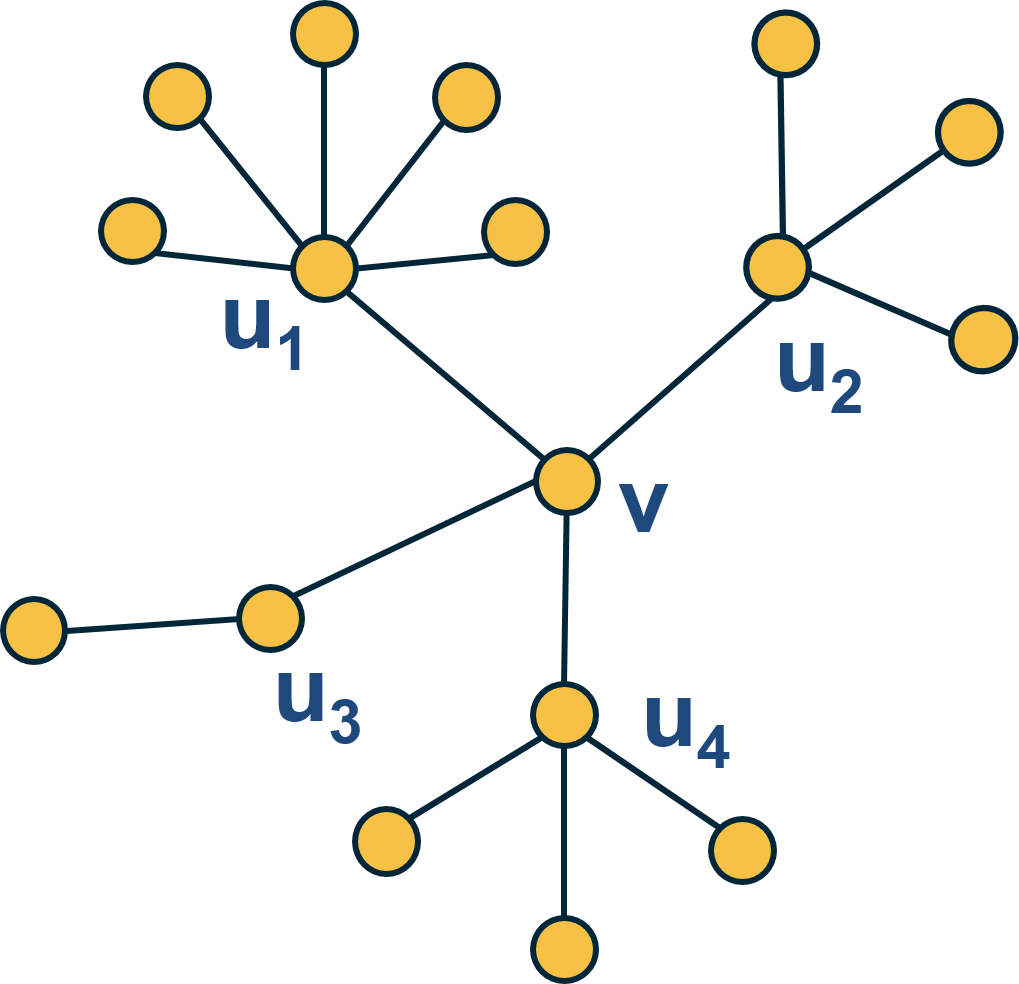
\includegraphics[width=0.5\linewidth]{k-neighbor-example.png}
    \caption{formula: $\overline{k_{nn}}(v)\:=\frac{\:1}{k(v)}\sum\limits_{i=1}^{k(v)}k(u_i)=\frac{6+4+2+4}{4}\:=\:4$}
\end{figure}

\subsection{Adjacency Matrix and List}
The adjacency list representation requires n+2*m space because every edge is included twice. 
\textbf{TODO adjacency matrix}

\section{Neutral Network}
Definition: the Degree of any two notes is not correlated.
\textbf{Most networks are not Neutral}
$k_{nn}(k)\:=\:\overline{k}+\frac{\sigma_k^2}{\overline{k}}=\bar{k}_{nn}$


Answer: The probability that a node does \textbf{not} connect to any node in the LCC $(1-p)^{S \, n}\approx(1-p)^n\:$if$\:S\approx1$

The expected number of nodes not connecting to LCC:
$\:n\cdot(1-p)^n\:=\:n(1-\frac{np}{n})^n\approx n\cdot e^{-n\cdotp}$

\subsection{classification of Networks}
\begin{description}
    \item[Scale Free] (TBC)
    \item[Neutra] (TBC)
\end{description}
$P_{edge}(k)= $Probability(given edge has degree k)$=\frac{kP(k)}{\overline{k}}$
Limit Definition of Exponential Function $(1-\frac{x}{n})^n\approx e^{-x}$
\subsection{links}
\href{https://en.wikipedia.org/wiki/Erd%C5%91s%E2%80%93R%C3%A9nyi_model}{wikipedia}\\
\href{https://en.wikipedia.org/wiki/Binomial_distribution}{Binomial distribution}\\
The Puissant distribution is a good approximation when $n>1,000$

\end{document}
